制导是导引和控制飞行器按一定规律飞向目标或预定轨道的技术和方法。
制导过程中,系统不断无人机与目标或预定轨道的相对位置关系,发出制导信息传递给姿态控制器,以控制飞行. 控制方式如图\ref{fig:posi}所示.
\begin{figure}[htbp]
        \centering
        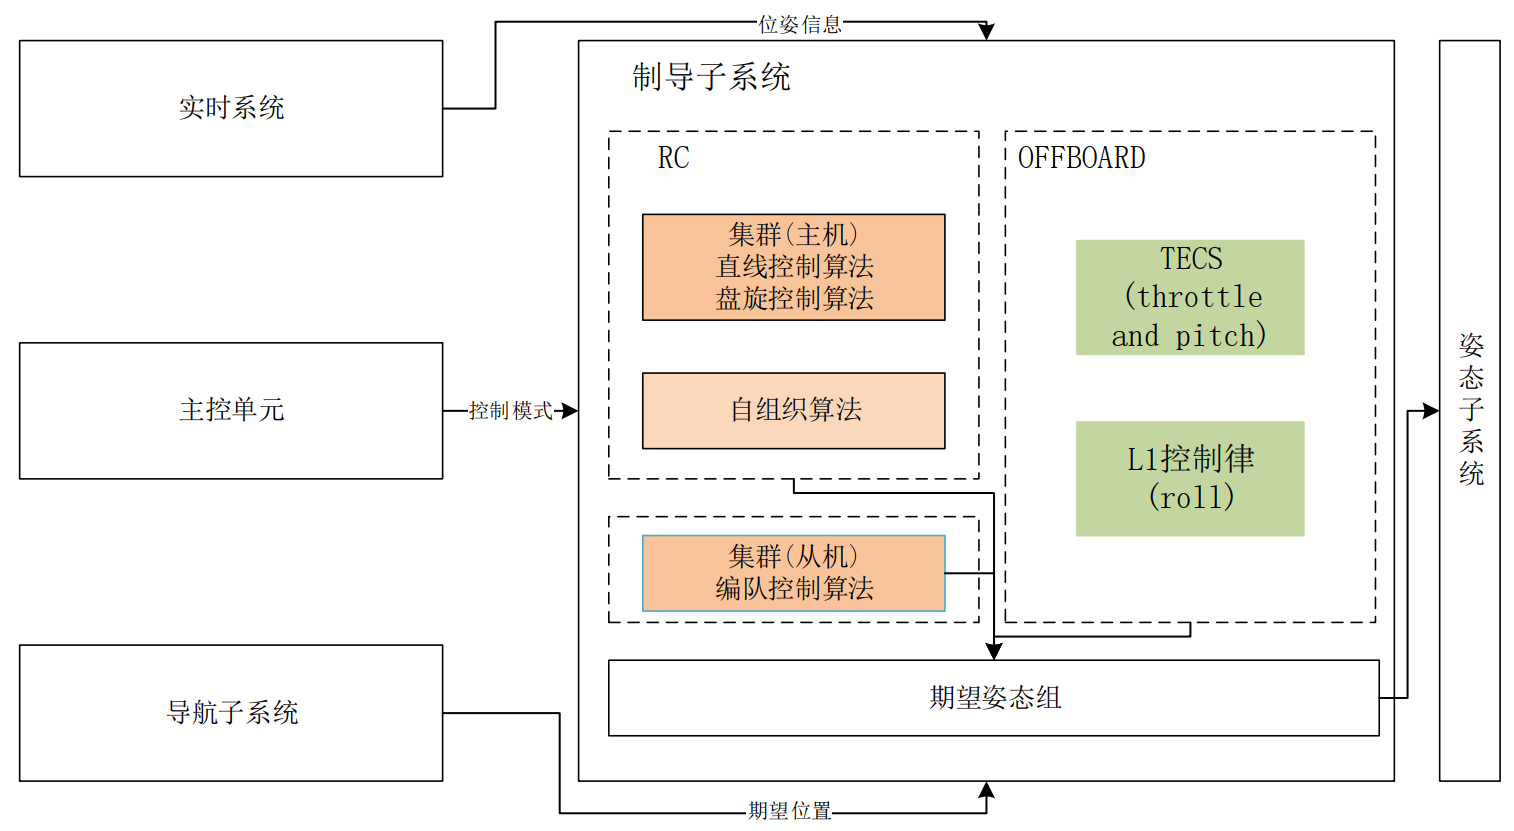
\includegraphics[width=\textwidth]{pictures/positionCtrl.png}
        \caption{position controller}
        \label{fig:posi}
    \end{figure}
\par 数据准备阶段有从实时系统获取当前的位姿信息, 从主控模块获取控制模式, 以及从导航子系统中获取期望位置. 之后的数据处理阶段主要有两套逻辑: 单机和集群两种处理模式; 
其中单机处理模式又分为 RC处理模式(ALTCTL), 以及OFFBOARD处理模式; 集群有编队控制模式. 
\par 
RC处理模式下, 有直线控制逻辑, 盘旋控制逻辑, 以及自组织控制逻辑; OFFBOARD处理模式下, 有总能量守恒(TECS)以及L1控制律. 在集群编队控制中, 有编队控制算法. 在各种算法的计算下, 可以得到期望姿态组, 有欧拉角(roll, pitch, yaw)设定值, 以及油门(throttle)设定值. 
进而下发给姿态子系统. 

% 数据的整合方法